\documentclass[a4paper,10pt]{article}
\usepackage[utf8]{inputenc}
\usepackage[final]{pdfpages}
\usepackage{caption}

\newcommand{\fw}{\linewidth}

\title{Math 660: Problem Set 5}
\author{Matthew Grasinger}

\begin{document}
  \maketitle

	\section{C1: ADI}
	
	The relative $L_\infty$ errors for $k = h = \frac{1}{10}, \frac{1}{20}$ and $\frac{1}{40}$ were 0.00163, 0.000476, and 0.000161, respectively.
	This means that, roughly, each time $k$ and $h$ were halved the error decreased by a factor of four.
	This suggests that the approximation accuracy is second order, which agrees with the theory.
	In the three figures that follow, the ADI approximation is compared with the exact solution.
	The approximation agrees well with the exact solution in all cases.

{
	\centering
	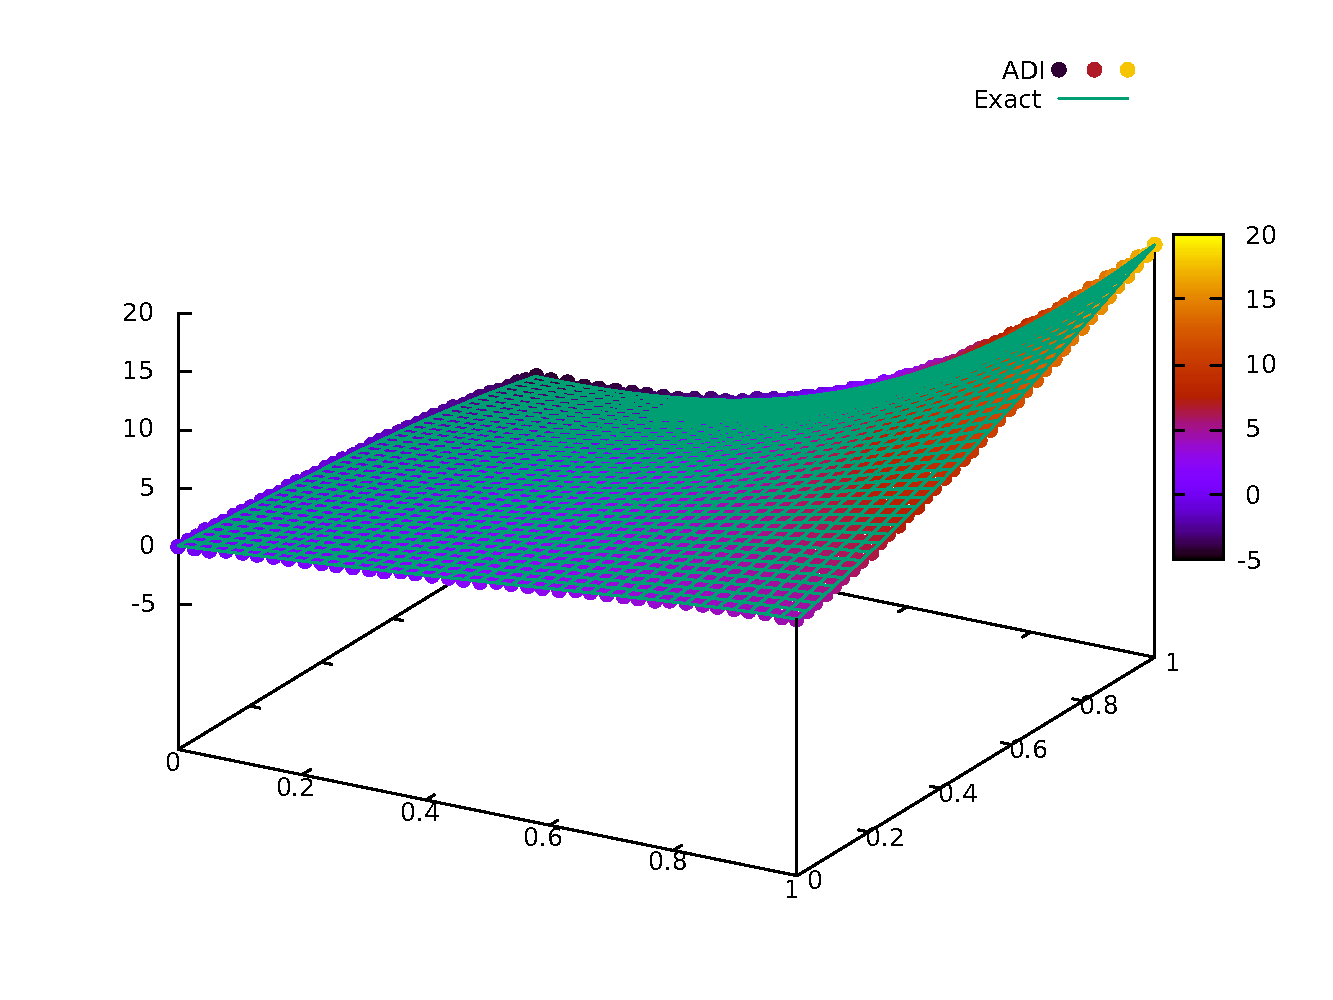
\includegraphics[width=\fw]{h-0100}
	\captionof{figure}{ADI approximation compared with exact solution. $h = \frac{1}{10}$.}
	\vspace{0.25in}
	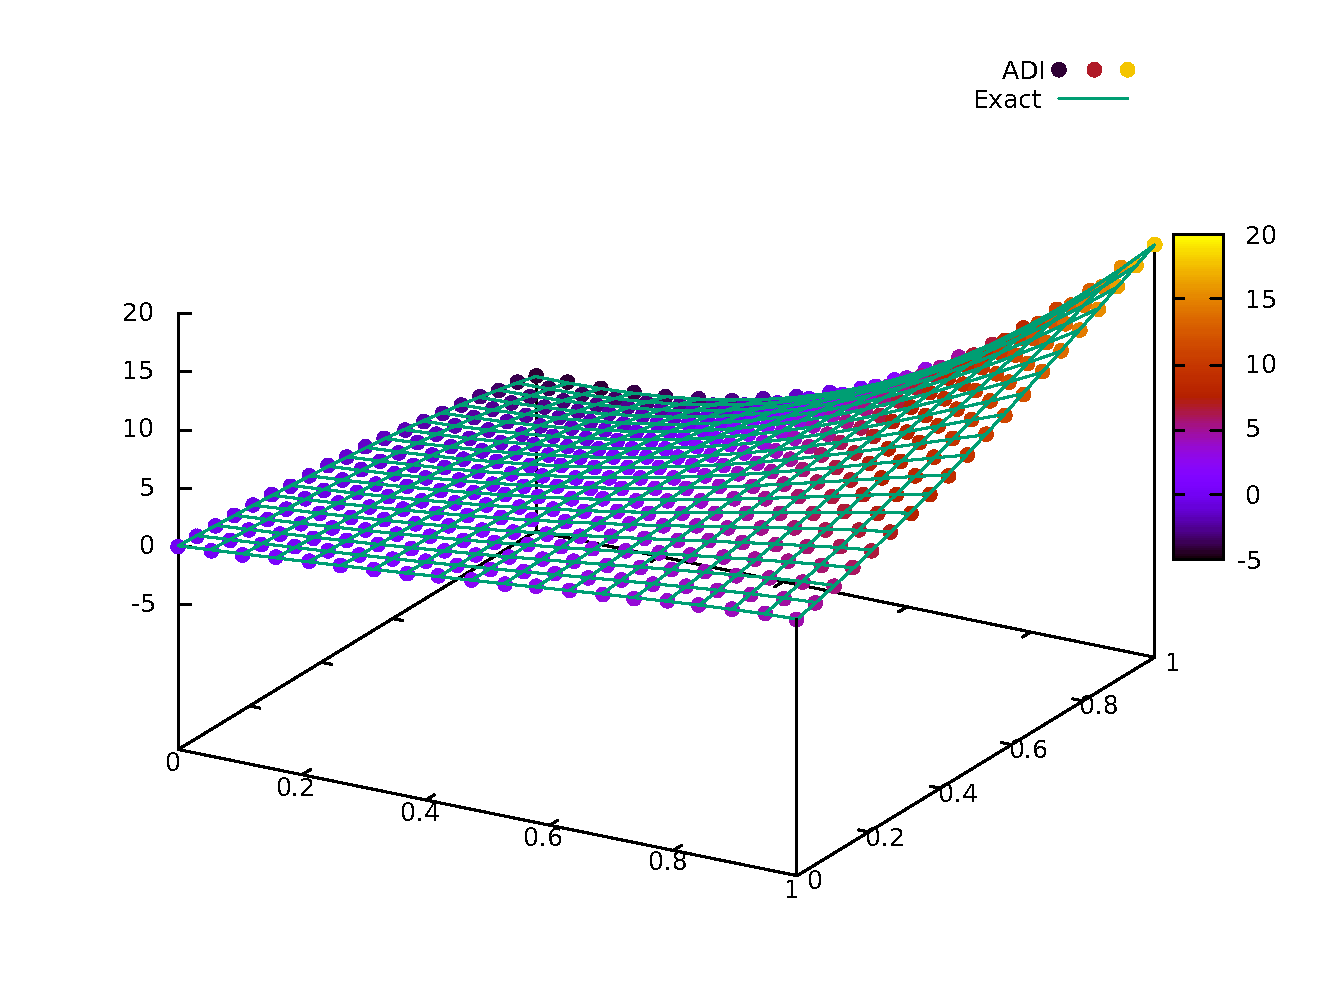
\includegraphics[width=\fw]{h-0050}
	\captionof{figure}{ADI approximation compared with exact solution. $h = \frac{1}{20}$.}
	\vspace{0.25in}
	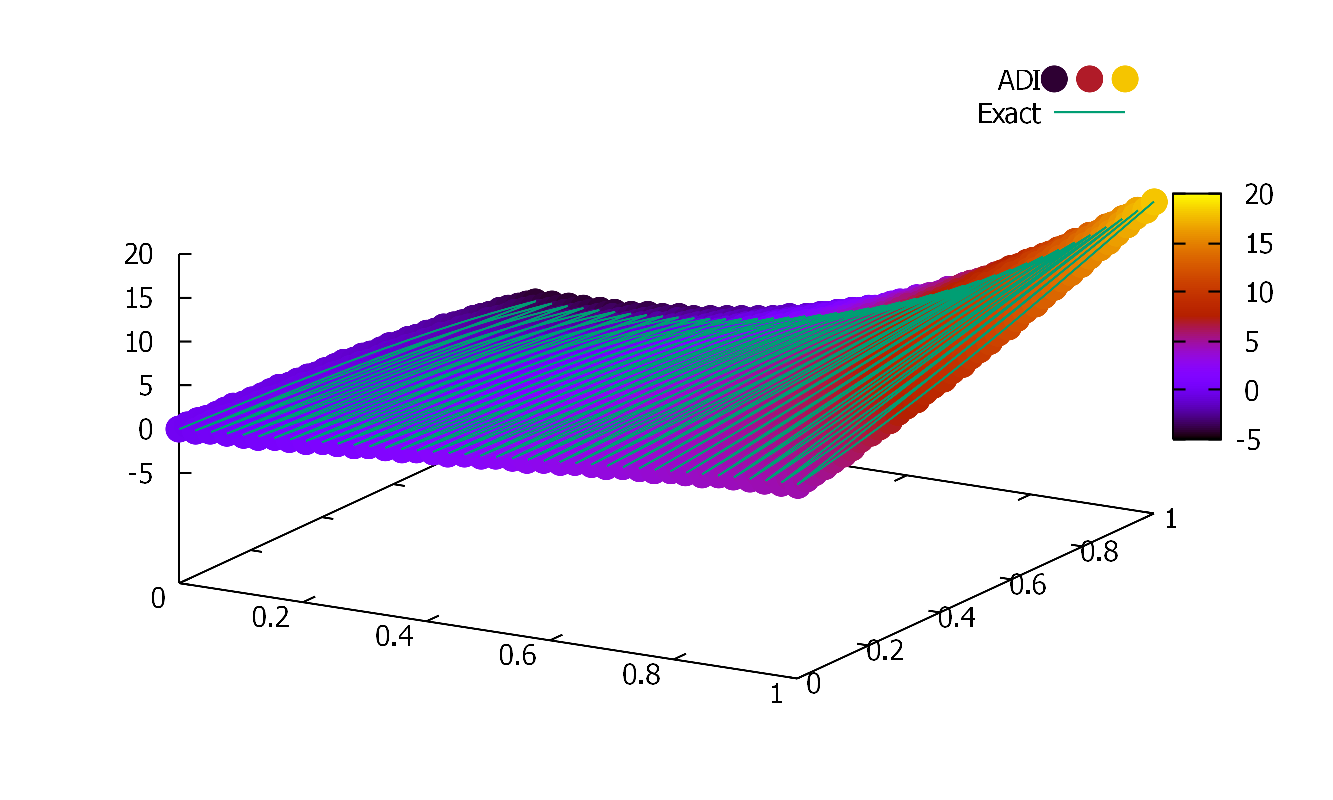
\includegraphics[width=\fw]{h-0025}
	\captionof{figure}{ADI approximation compared with exact solution. $h = \frac{1}{40}$.}
	\vspace{0.25in}
}
		
	\subsection{Source Code}
	
	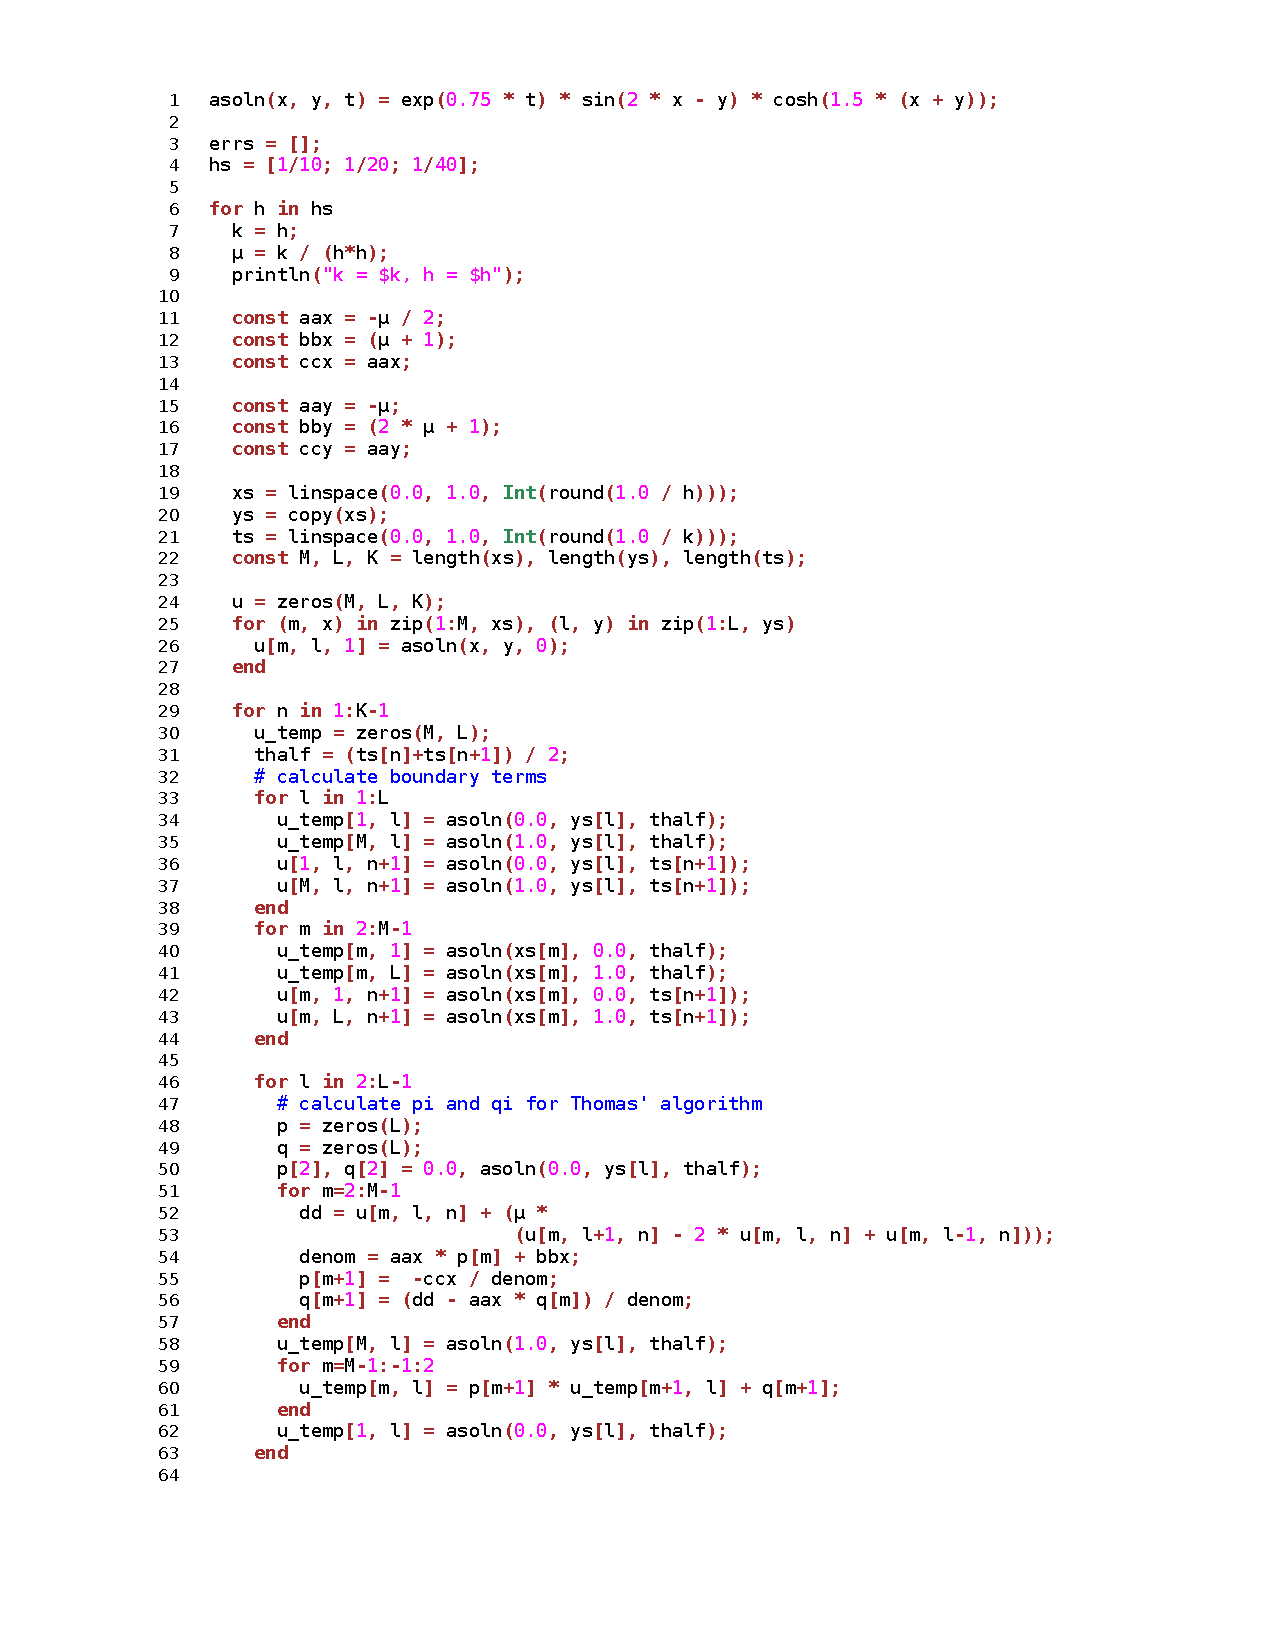
\includepdf[pages=-]{./hw5_code.pdf}
	
	\section{Douglas-Rachford (Optional)}
	
	For the Douglas-Rachford scheme the grid spacings were $h = \frac{1}{10}, \frac{1}{20}$ and $\frac{1}{40}$, but $k$ was taken to be $k = h^2$ because the Douglas-Rachford scheme is second order accurate in space but only first order accurate in time.
	The relative $L_\infty$ errors for $h = \frac{1}{10}, \frac{1}{20}$ and $\frac{1}{40}$ were 0.00114, 0.000393, and 0.000314, respectively.
	Notice that, roughly, when $h$ was halved the first time (from $h = \frac{1}{10}$ to $h = \frac{1}{20}$ and $k = \frac{1}{100}$ to $k = \frac{1}{400}$) the error decreased by a factor of four, which agrees with the theory.
	However, when $h$ was halved again there were diminishing returns on the accuracy as the accuracy only increased by less than 25\%.
	In the three figures that follow, the ADI approximation is compared with the exact solution.
	The approximation agrees well with the exact solution in all cases.
	
	{
		\centering
		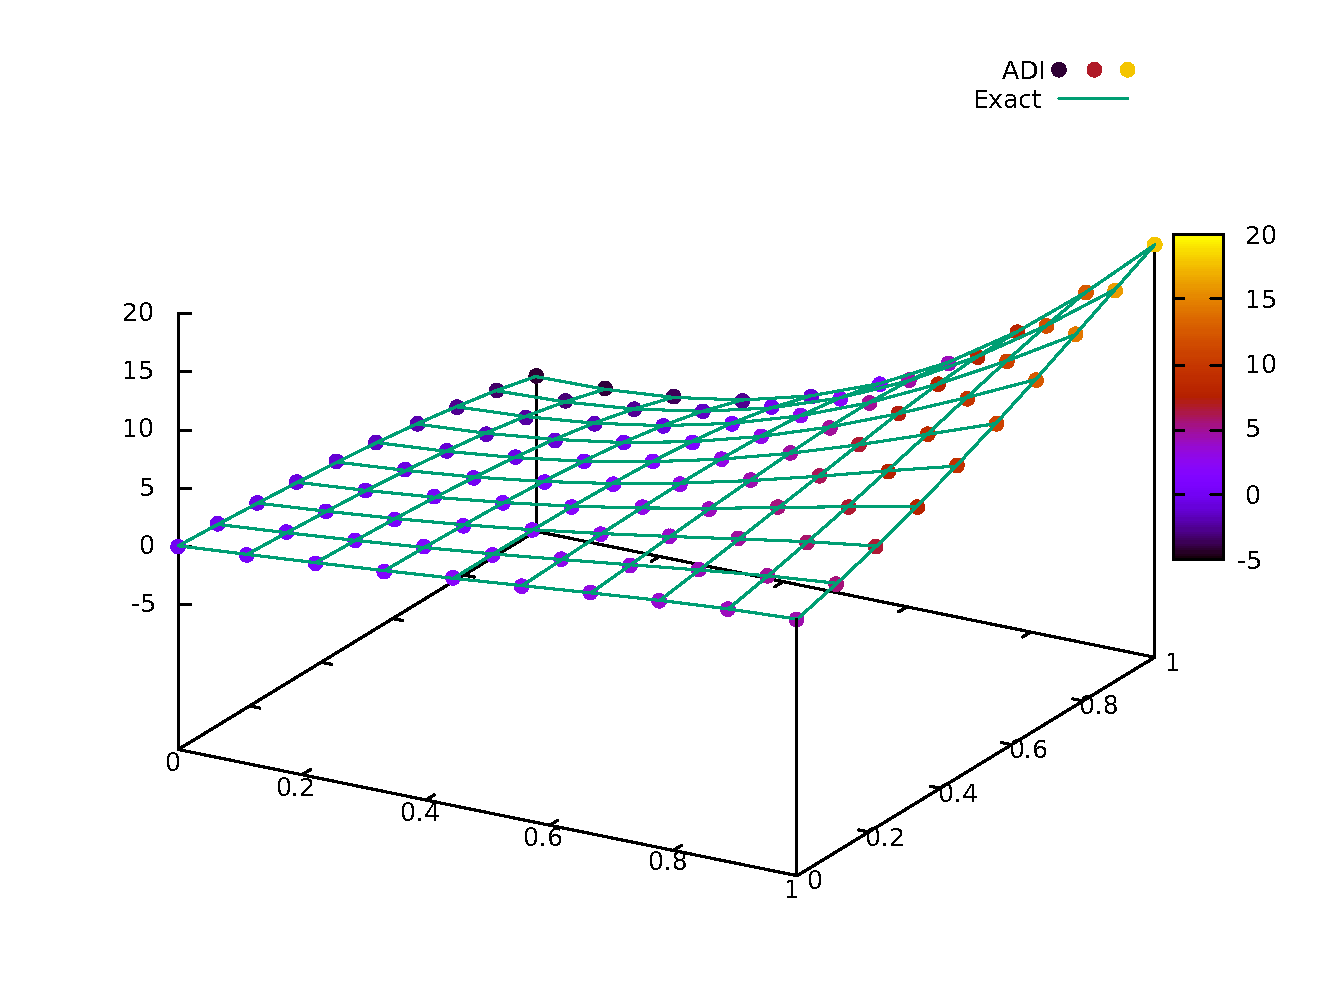
\includegraphics[width=\fw]{h-0100_dr}
		\captionof{figure}{ADI approximation compared with exact solution. $h = \frac{1}{10}$, $k = \frac{1}{100}$.}
		\vspace{0.25in}
		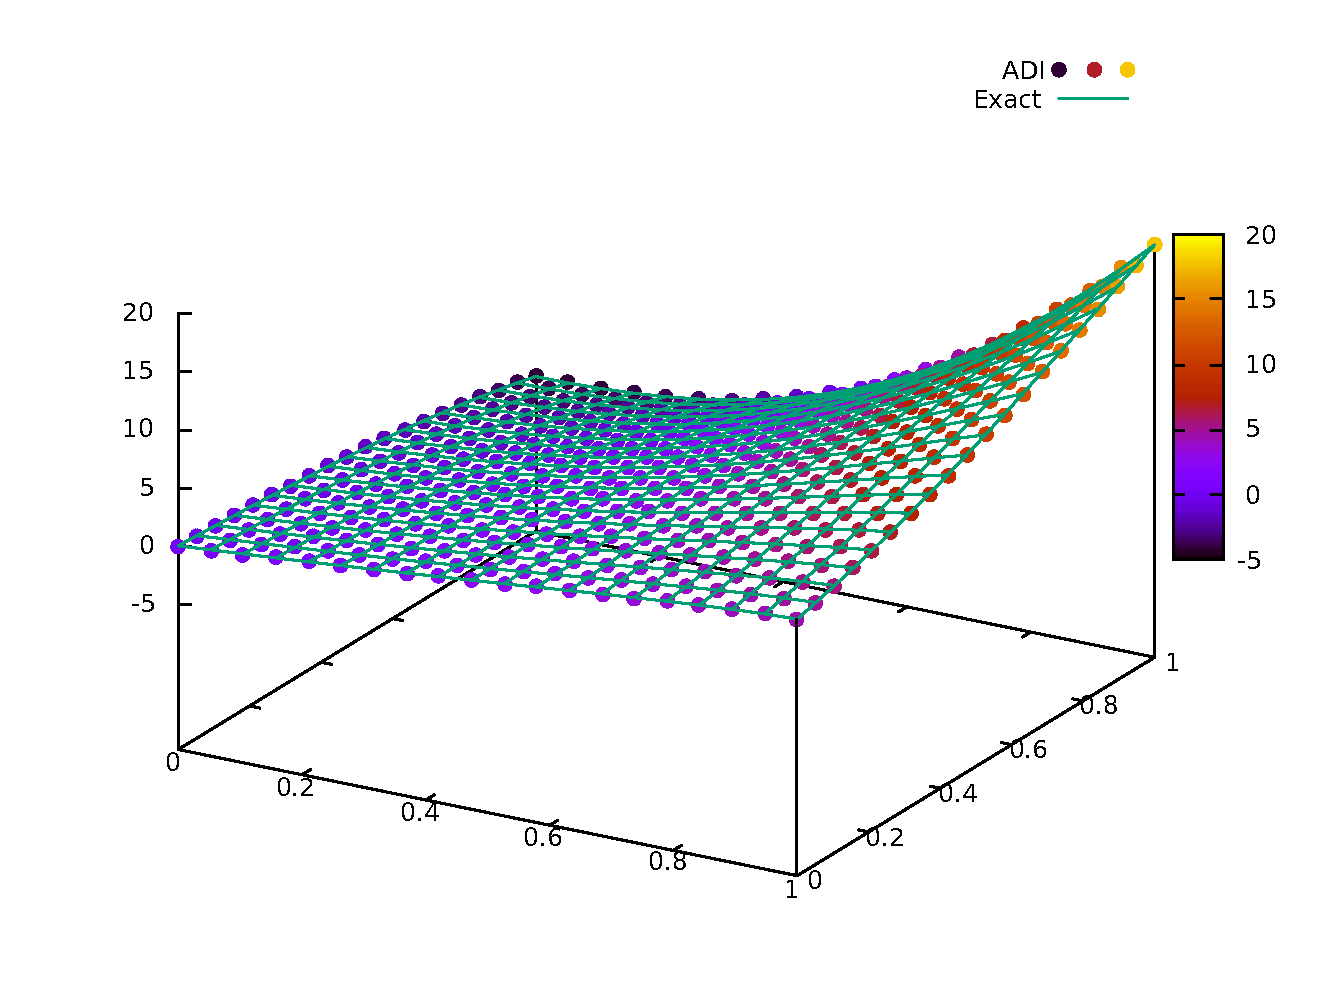
\includegraphics[width=\fw]{h-0050_dr}
		\captionof{figure}{ADI approximation compared with exact solution. $h = \frac{1}{20}$, $k = \frac{1}{400}$.}
		\vspace{0.25in}
		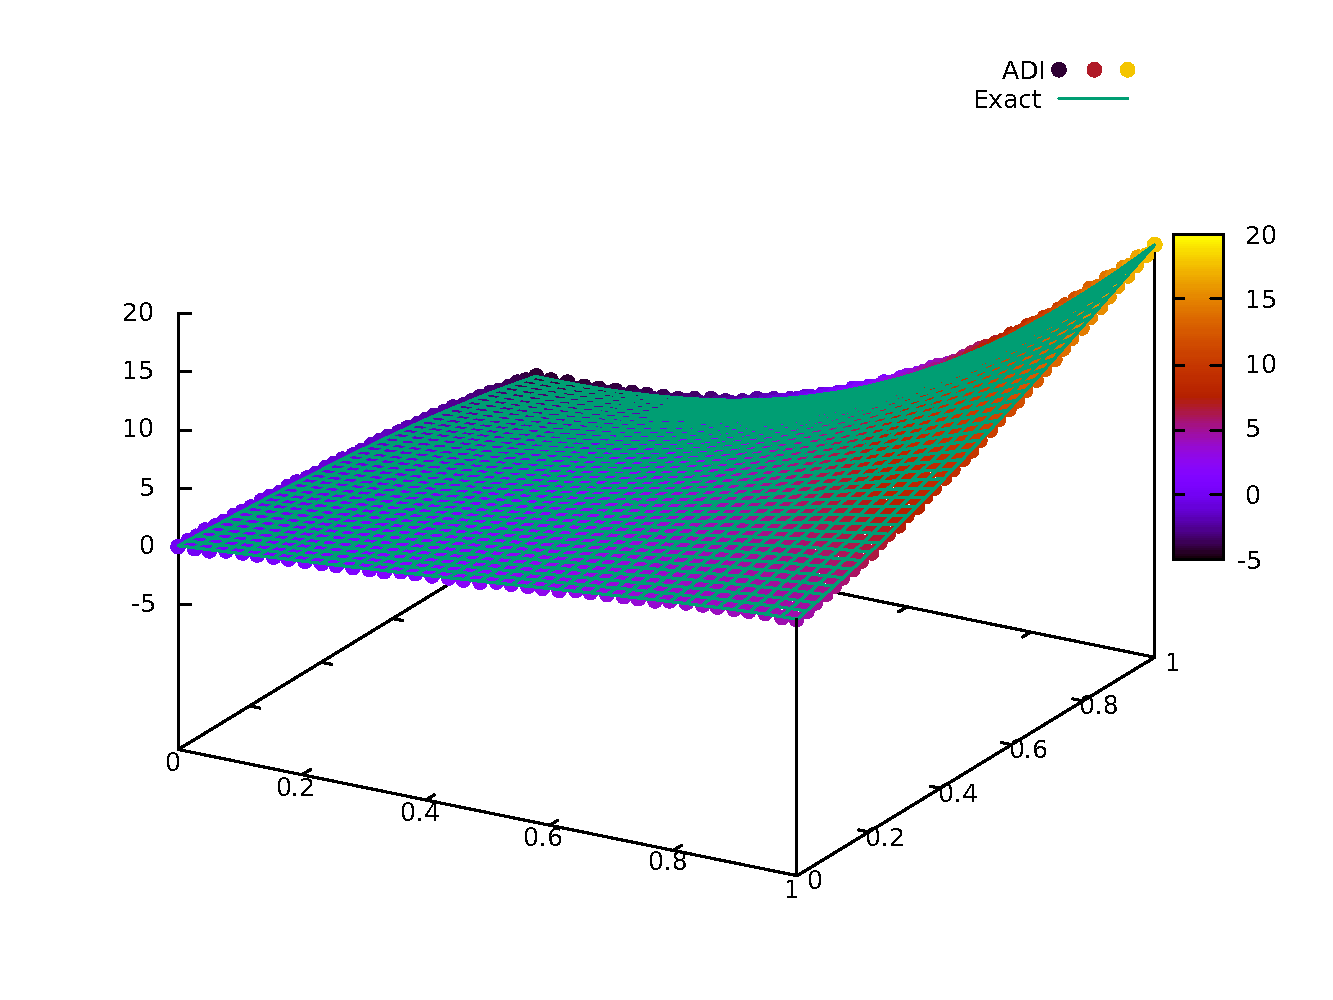
\includegraphics[width=\fw]{h-0025_dr}
		\captionof{figure}{ADI approximation compared with exact solution. $h = \frac{1}{40}$, $k = \frac{1}{1600}$.}
		\vspace{0.25in}
	}
	
	\subsection{Source Code}
	
	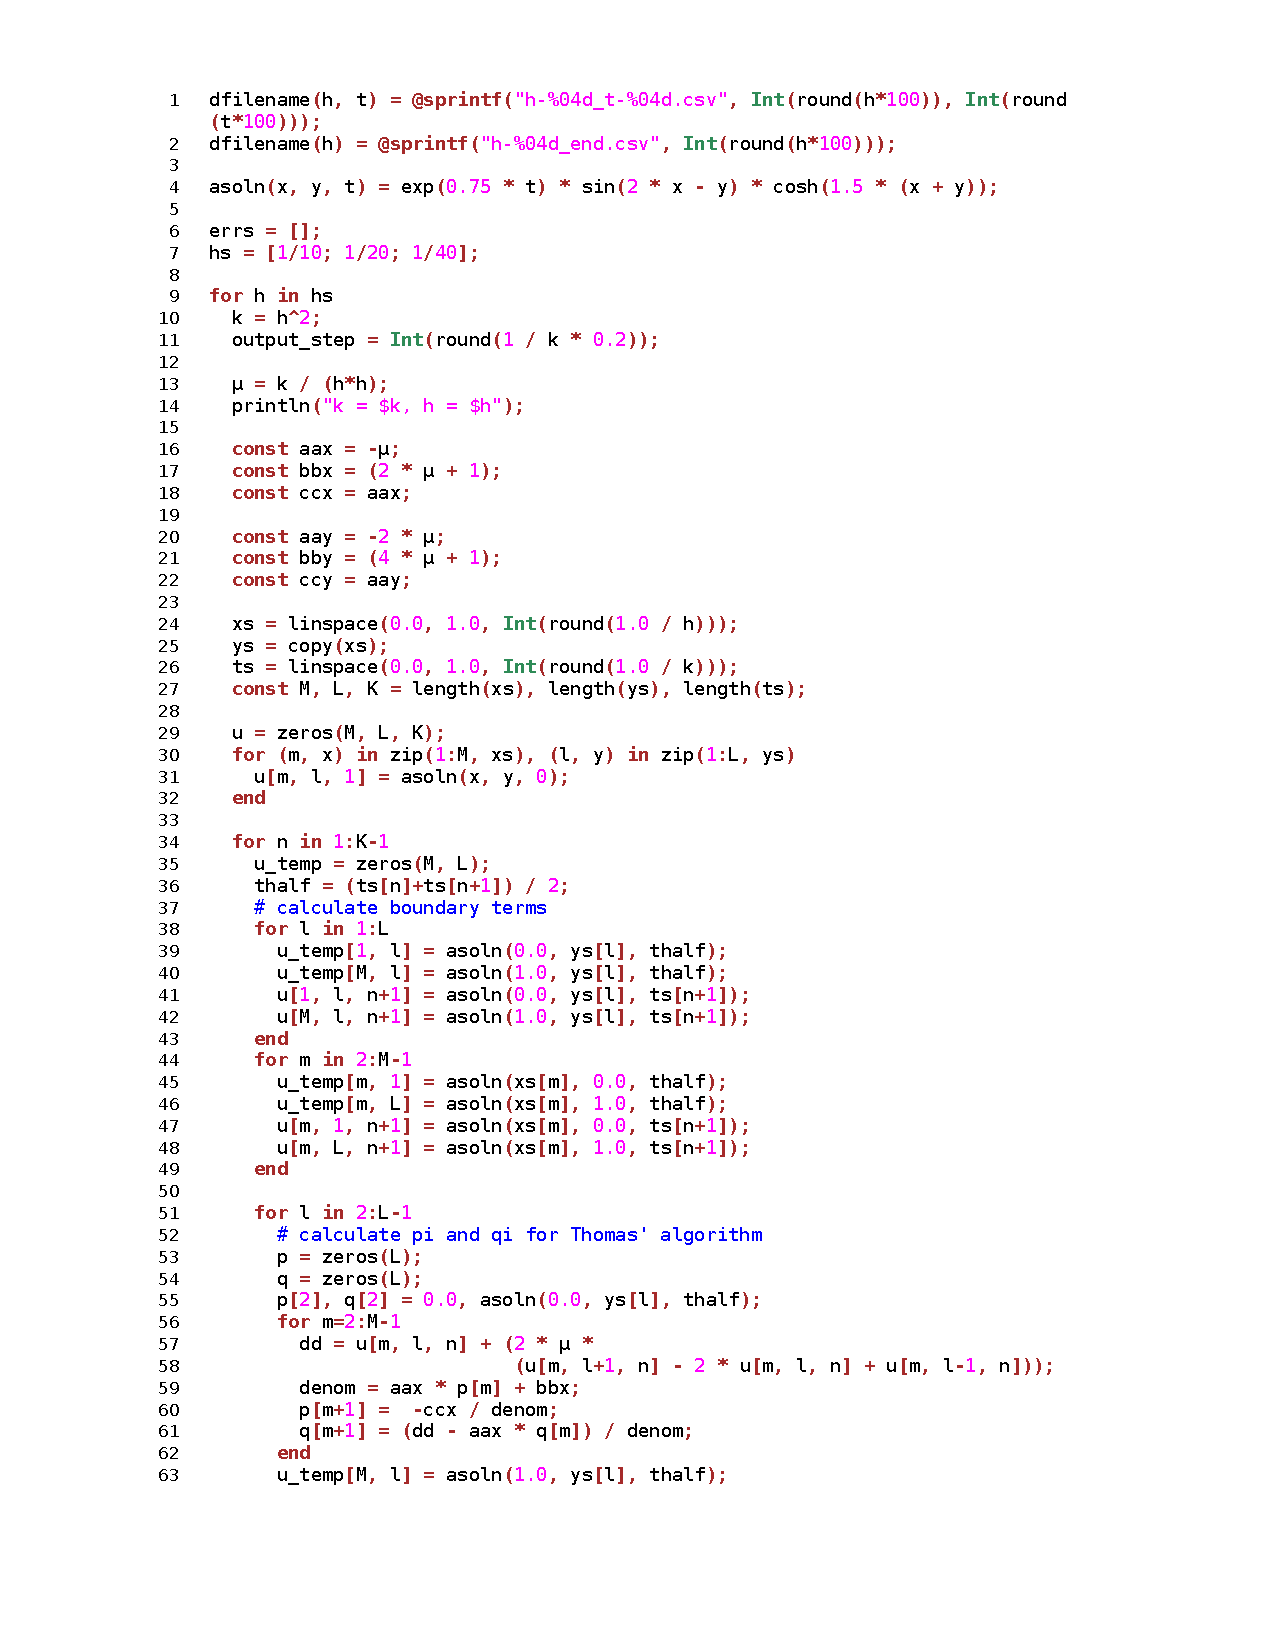
\includepdf[pages=-]{./hw5dr.pdf}
\end{document}
